%Dr. Shriram Jois
\documentclass[a4paper,11pt]{extarticle}
\usepackage[utf8]{inputenc}
\usepackage{setspace}
\usepackage{graphicx}
\usepackage{pgfgantt}
\usepackage{caption}
\usepackage{subcaption}
\usepackage{hyperref}
\usepackage{enumitem}
\usepackage{geometry}
 \geometry{
 a4paper,
 left=17mm,
 top=18mm,
 }
 \singlespacing
 
%page number
\usepackage{fancyhdr}
\usepackage{lastpage}
\pagestyle{fancy}
\fancyhf{}
\lhead{Standard EF}
\chead{Project Title - ProT}
\rhead{Page \thepage \hspace{1pt} of \pageref{LastPage}}

%Header and footer rule width
\renewcommand{\headrulewidth}{2pt}
%\renewcommand{\footrulewidth}{1pt}

\renewcommand{\footnotesize}{\fontsize{8pt}{8pt}\selectfont}

\title{Axion Search in DarkSide-20k (ASiD)}
\author{Shriram Sadashivajois}
\date{\today}

%\bibliographystyle{unsrt}
%\bibliographystyle{bst/apsrev4-2}

\begin{document}

%\maketitle

\section{Excellence}
\subsection{Quality and credibility of the research; level of novelty, appropriate consideration of inter/multidisciplinary and gender aspects}
\subsubsection{Introduction to dark matter}
Adding a reference under a footnote - \footnote{A. Awesome et. al, Abbr. J. name \textbf{volume number}, page number in regular font (Year of publication).\label{footnote1}} 
\\ \\
Citing a previous added footnote - \footref{footnote1}.
\\ \\
Do not forget to end an equation either with a comma or a fullstop.

\subsubsection{Solar axion as a hot dark matter candidate}
\subsubsection{Dark matter search in DarkSide-20k}
\subsubsection{Novelty and State-of-the-art}
I plan to organize the project in three work packages and each work package is organized in three tasks.
%\begin{itemize}
    %\setlength\itemsep{0em}
    %\item incorporating energy
    %\item going beyond the state-of-the-art by using the Si in the SiPM detector itself as a target for dark matter for the first time.
    %\item using the Si in the SiPM detector to study the diurnal and annual modulation of WIMPs.
%\end{itemize}
\subsubsection{Proposed work packages for the proposal}
\textbf{Work package 1} 
\begin{itemize}
    \setlength\itemsep{-0.2em}
    \item \textit{Task 1}: 
    \item \textit{Task 2}: 
    \item \textit{Task 3}: 
\end{itemize}
\textbf{Work package 2} 
\begin{itemize}
    \setlength\itemsep{-0.2em}
    \item \textit{Task 1}: 
    \item \textit{Task 2}: 
    \item \textit{Task 3}: 
\end{itemize}
\textbf{Work package 3} 
\begin{itemize}
    \setlength\itemsep{-0.2em}
    \item \textit{Task 1}: 
    \item \textit{Task 2}: 
    \item \textit{Task 3}: 
\end{itemize}
\subsubsection{Multidisciplinary and collaboration opportunities}
The project would provide me an opportunity to work on . . .
\begin{itemize}
\setlength\itemsep{-0.2em}
    \item Physics + engineering bigger picture.
    \item Cryogenics.
    \item Data analysis. 
    \item A small note on workshops and conferences.
\end{itemize}
\subsubsection{Gender aspects in my research}
\subsection{Quality and appropriateness of the training and of the two way transfer of knowledge between the researcher and the host}
\subsubsection{Quality and appropriateness of training of the researcher}
I used both paragraphs and bullets \begin{itemize}
    \item where ever,
    \item necessary.
\end{itemize}
\subsubsection{Transfer of two way knowledge}
I used both paragraphs and bullets \begin{itemize}
    \item where ever,
    \item necessary.
\end{itemize}
\subsection{Quality of the supervision and of the integration in the team/institution}
I used both paragraphs and bullets \begin{itemize}
    \item where ever,
    \item necessary.
\end{itemize}
\subsection{Potential of the researcher to reach or re-enforce professional maturity during the fellowship}
\section{Impact}
\subsection{Enhancing the potential and future career prospects of the researcher}
\subsection{Quality of the proposed measures to exploit and disseminate the action results}
\subsection{Quality of the proposed measures to communicate the project activities to different target audiences}
\section{Implementation}
\subsection{Coherence and effectiveness of the work plan, including appropriateness of the allocation of tasks and resources}
There are online notes on writing a gantt with creative touch.\footnote{Wolfgang Skala, \href{https://texdoc.org/serve/pgfgantt/0}{https://texdoc.org/serve/pgfgantt/0}}
\\ \\
\begin{tabular}{ |p{2cm}|p{6cm}|p{6.8cm}| }
 \hline
 \multicolumn{3}{|c|}{Project plan} \\
 \hline
 Work package number & Task & Deliverable (D) and Milestone (M)\\
 \hline
 1 & 1.  & D1.1 ; M1.1 .  \\
 \hline
 1 & 2.  & D1.2 ; M1.2 .\\
 \hline
 1 & 3.  & M1.3 \\
 \hline
 2 & 1.  & D2.1 ; M2.1  \\ 
 \hline
 2 & 2.  & M2.2 \\
 \hline
 2 & 3.  & D2.3 \\
 \hline
 3 & 1.  & D3.1 \\
 \hline
 3 & 2.  & D3.2 ; M3.2 \\
 \hline
 3 & 3.  & D3.3 ; M3.3  \\
 \hline
 4 & 1.  & M4.1 \\
 \hline
 5 & 1. Dissemination and outreach & D5.1 Publications and talks; D5.2 Dark matter outreach; M5.1 My first public lecture. \\
\hline
\end{tabular}
\\ \\
In the table, task 1.1 corresponds to the task number 1 of work package 1. Work packages 4 and 5 are shown here as secondment, and conference and outreach. My original proposal contained a gantt chart made from Excel. I honed my writing skills in the past couple of years to write the chart in Latex. Fig. \ref{gantt_chart} is an example gantt chart. You will need pgfgantt package for the chart.
\begin{figure}
  \begin{ganttchart}[y unit title=0.38cm,
    y unit chart=0.43cm,
    vgrid,hgrid, 
    title label anchor/.style={below=-1.6ex},
    title left shift=.05,
    title right shift=-.05,
    title height=1,
    progress label text={},
    bar height=0.7,
    group right shift=0,
    group top shift=.6,
    group height=.3]{1}{24}
    %\gantttitle{June 2024 - May 2026}{24} \\
\gantttitle{2022}{12} 
\gantttitle{2023}{12} \\
\gantttitlelist{1,2,3,4,5,6,7,8,9,10,11,12}{1}
\gantttitlelist{1,2,3,4,5,6,7,8,9,10,11,12}{1}\\
%%%%%%%%%%%%%%%%%%%%%%%%%%%%%%%%%%

%First Group
%%%%%%%%%%%%%%%%%%%%%%%%%%%%%%%%%%

\ganttgroup{WP 1}{1}{11} \\
\ganttbar{Task name 1}{1}{5} \\  
\ganttbar{Task name 2}{6}{8} \\ 
\ganttbar{Task name 3}{9}{11} \\

%\ganttmilestone{Milestone 1}{11}\\

%\ganttlink{elem0}{elem1}
\ganttlink{elem1}{elem2} 
\ganttlink{elem2}{elem3} 
%%%%%%%%%%%%%%%%%%%%%%%%%%%%%%%%%%

%%%%%%%%%%%%%%%%%%%%%%%%%%%%%%%%%%

%\ganttmilestone{Milestone 1}{11}
%Second Group
%%%%%%%%%%%%%%%%%%%%%%%%%%%%%%%%%%
\ganttgroup{WP 2}{9}{17} \\
\ganttbar{Task name 1}{9}{11} \\
\ganttbar{Task name 2}{12}{17} \\
\ganttbar{Task name 3}{11}{15}\\
%\ganttmilestone{Milestone 2}{17}\\
\ganttlink{elem6}{elem7}
%%%%%%%%%%%%%%%%%%%%%%%%%%%%%%%%%%

%%%%%%%%%%%%%%%%%%%%%%%%%%%%%%%%%%

%\ganttmilestone{Milestone 1}{11}
%Third Group
%%%%%%%%%%%%%%%%%%%%%%%%%%%%%%%%%%
\ganttgroup{WP 3}{14}{24} \\
\ganttbar{Task name 1}{14}{17} \\
\ganttbar{Task name 2}{18}{20} \\
\ganttbar{Task name 3}{21}{24}

%\ganttmilestone{Milestone 3}{24}

\ganttlink{elem9}{elem10}
\ganttlink{elem9}{elem10}
\ganttlink{elem10}{elem11}
%%%%%%%%%%%%%%%%%%%%%%%%%%%%%%%%%%
\end{ganttchart}
\caption{The figure illustrates the project timeline using a gantt chart. I organized the project into WPs and subdivide the WPs into various tasks. When write your proposal make sure you switch the name of task with \textit{task name and number}.}
\label{gantt_chart}
\end{figure}
\subsection{Appropriateness of the management structure and procedures, including risk management}
\subsection{Appropriateness of the institutional environment (infrastructure)}
I illustrated the physics reach of the proposal with a picture at some point in the proposal, I think in the first section. You should be able to add multiple pictures with subfigure command.
\begin{figure}
\begin{subfigure}{.5\textwidth}
  \centering
  
\includegraphics[scale=0.07]{figures/teepee_1.jpg}
  \caption{The official portrait of TeePee. 
  }
  \label{fig:teepee_1}
\end{subfigure}%
\begin{subfigure}{.5\textwidth}
  \centering
  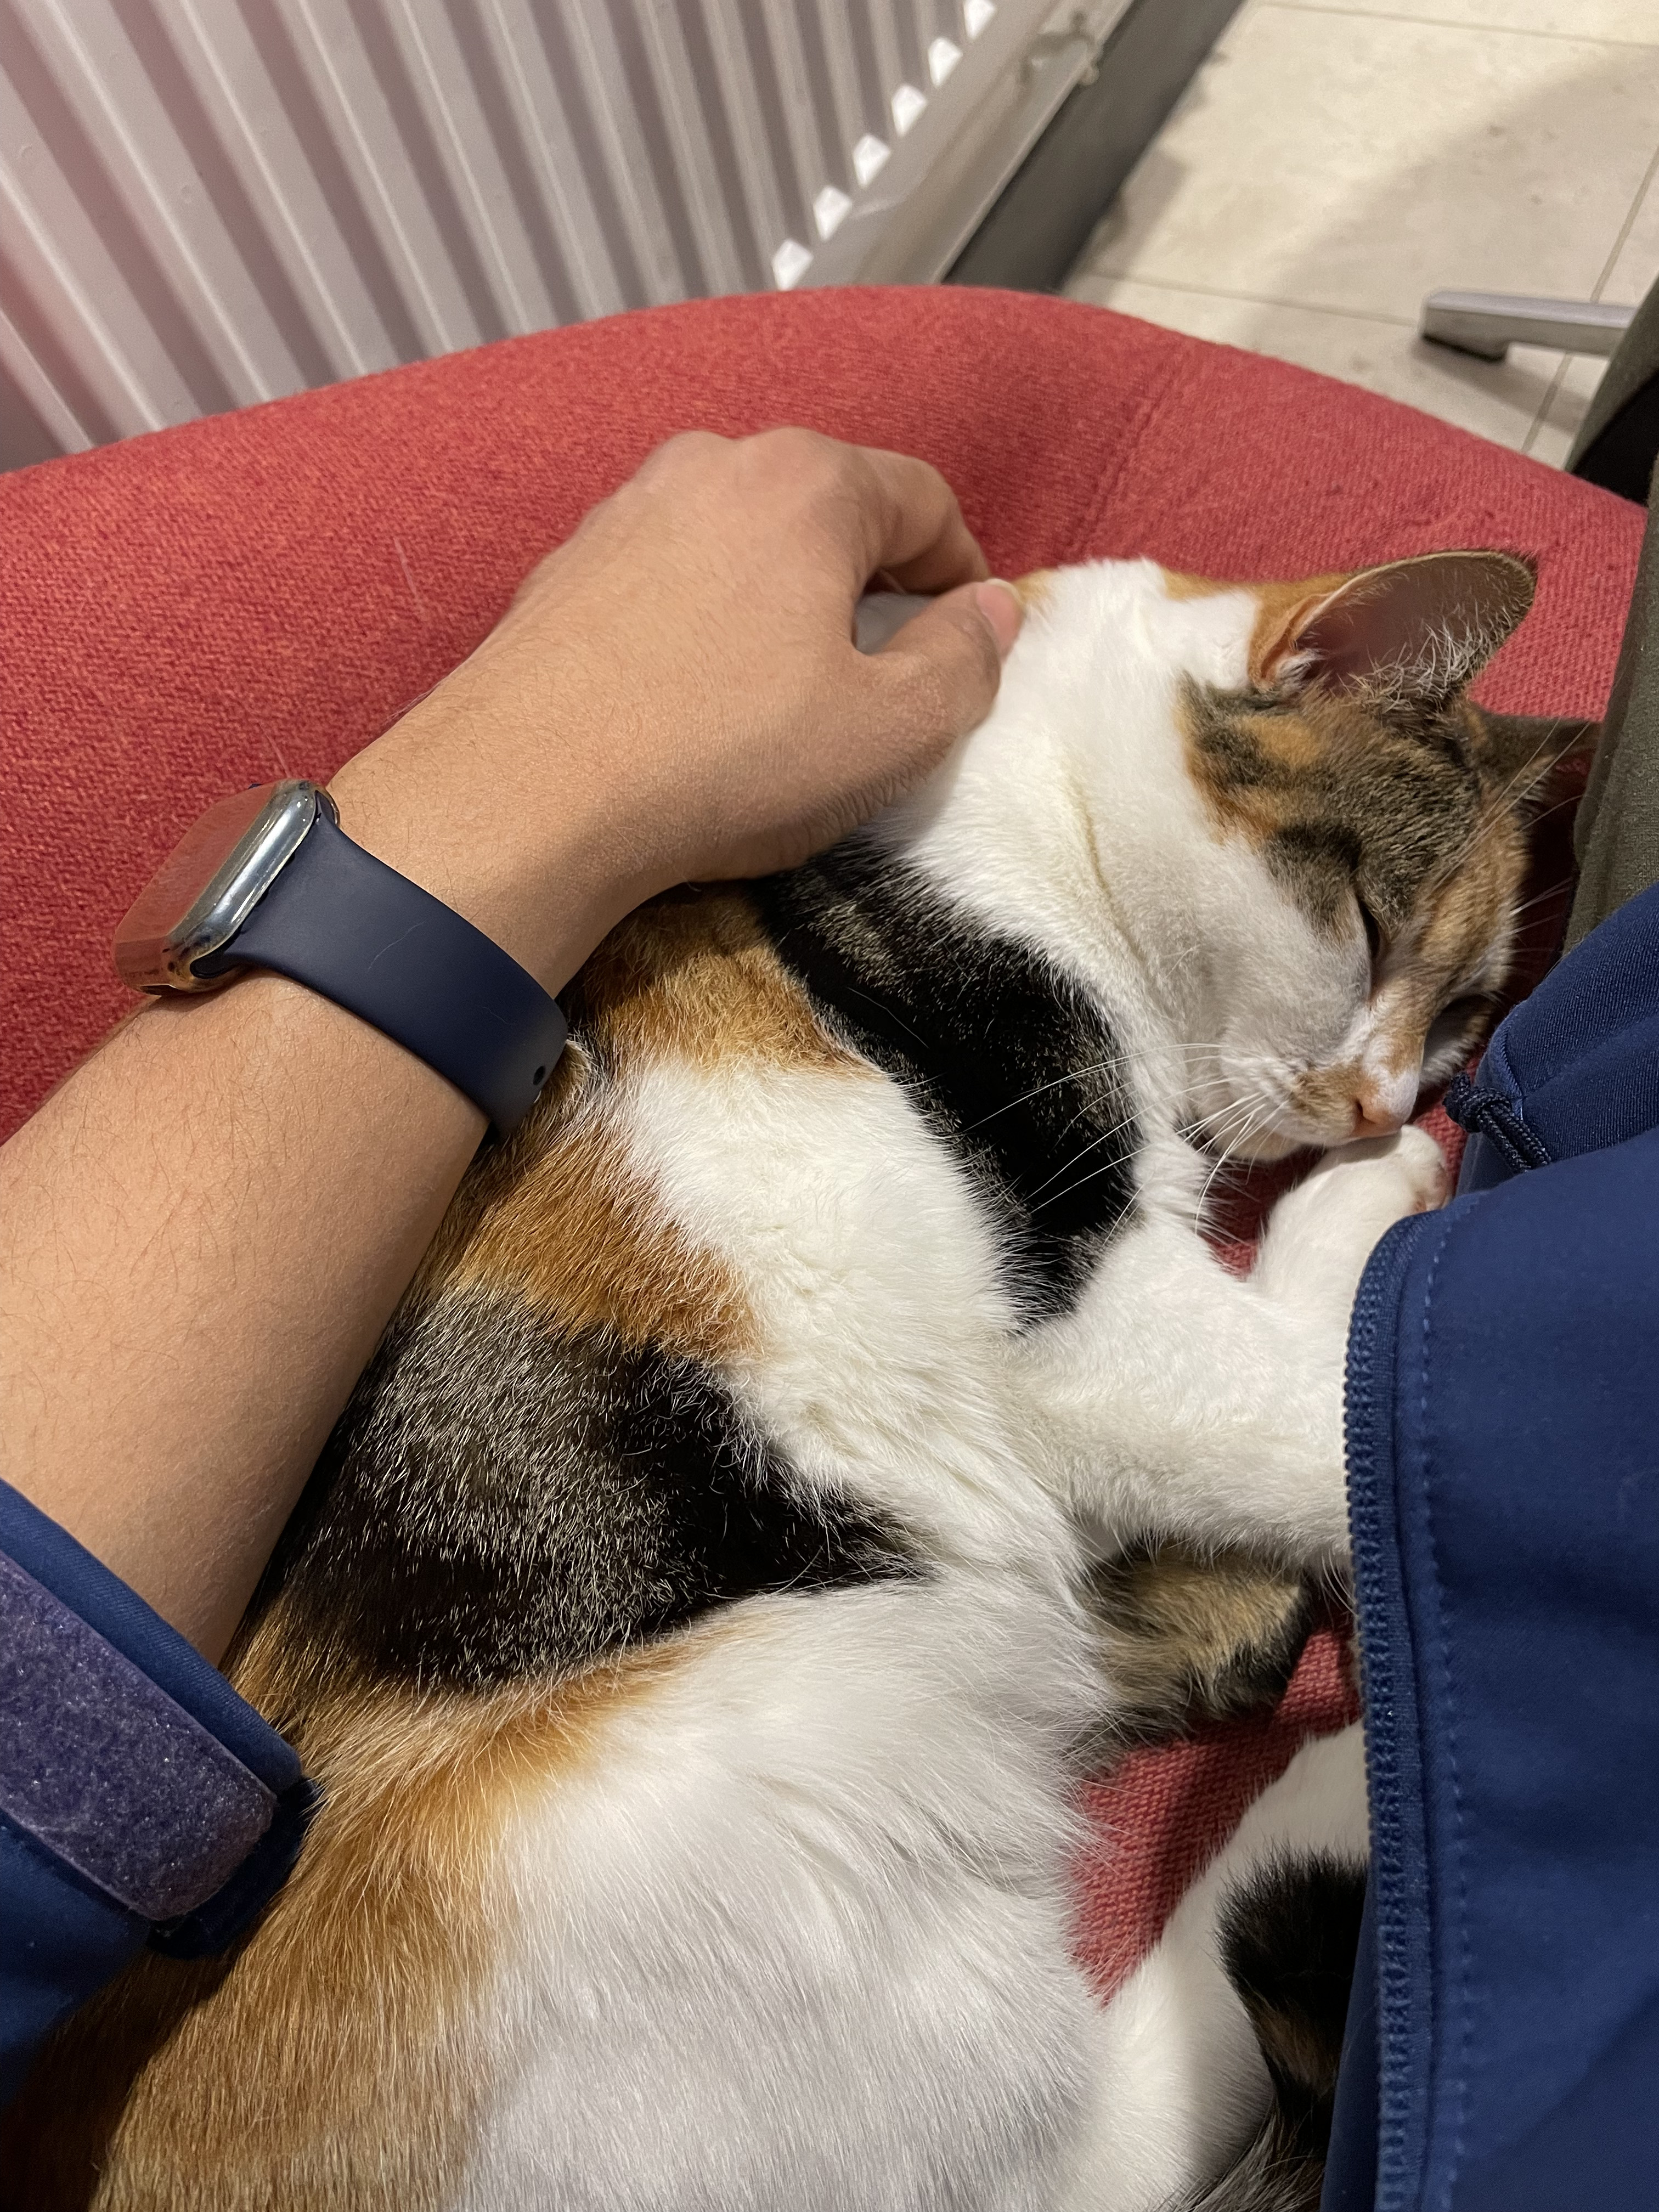
\includegraphics[scale=0.07]{figures/teepee_2.jpg}
  \caption{A therapeutic session with TeePee.}
  \label{fig:teepee_2}
\end{subfigure}
\caption{A stray cat can show more empathy towards you than your colleagues and supervisors in the UK.}
\label{fig:fig}
\end{figure}
\end{document}